\appendix

\section{Detailed Explanations for the Dependency Rules}
\begin{figure}[h]
    \centering
    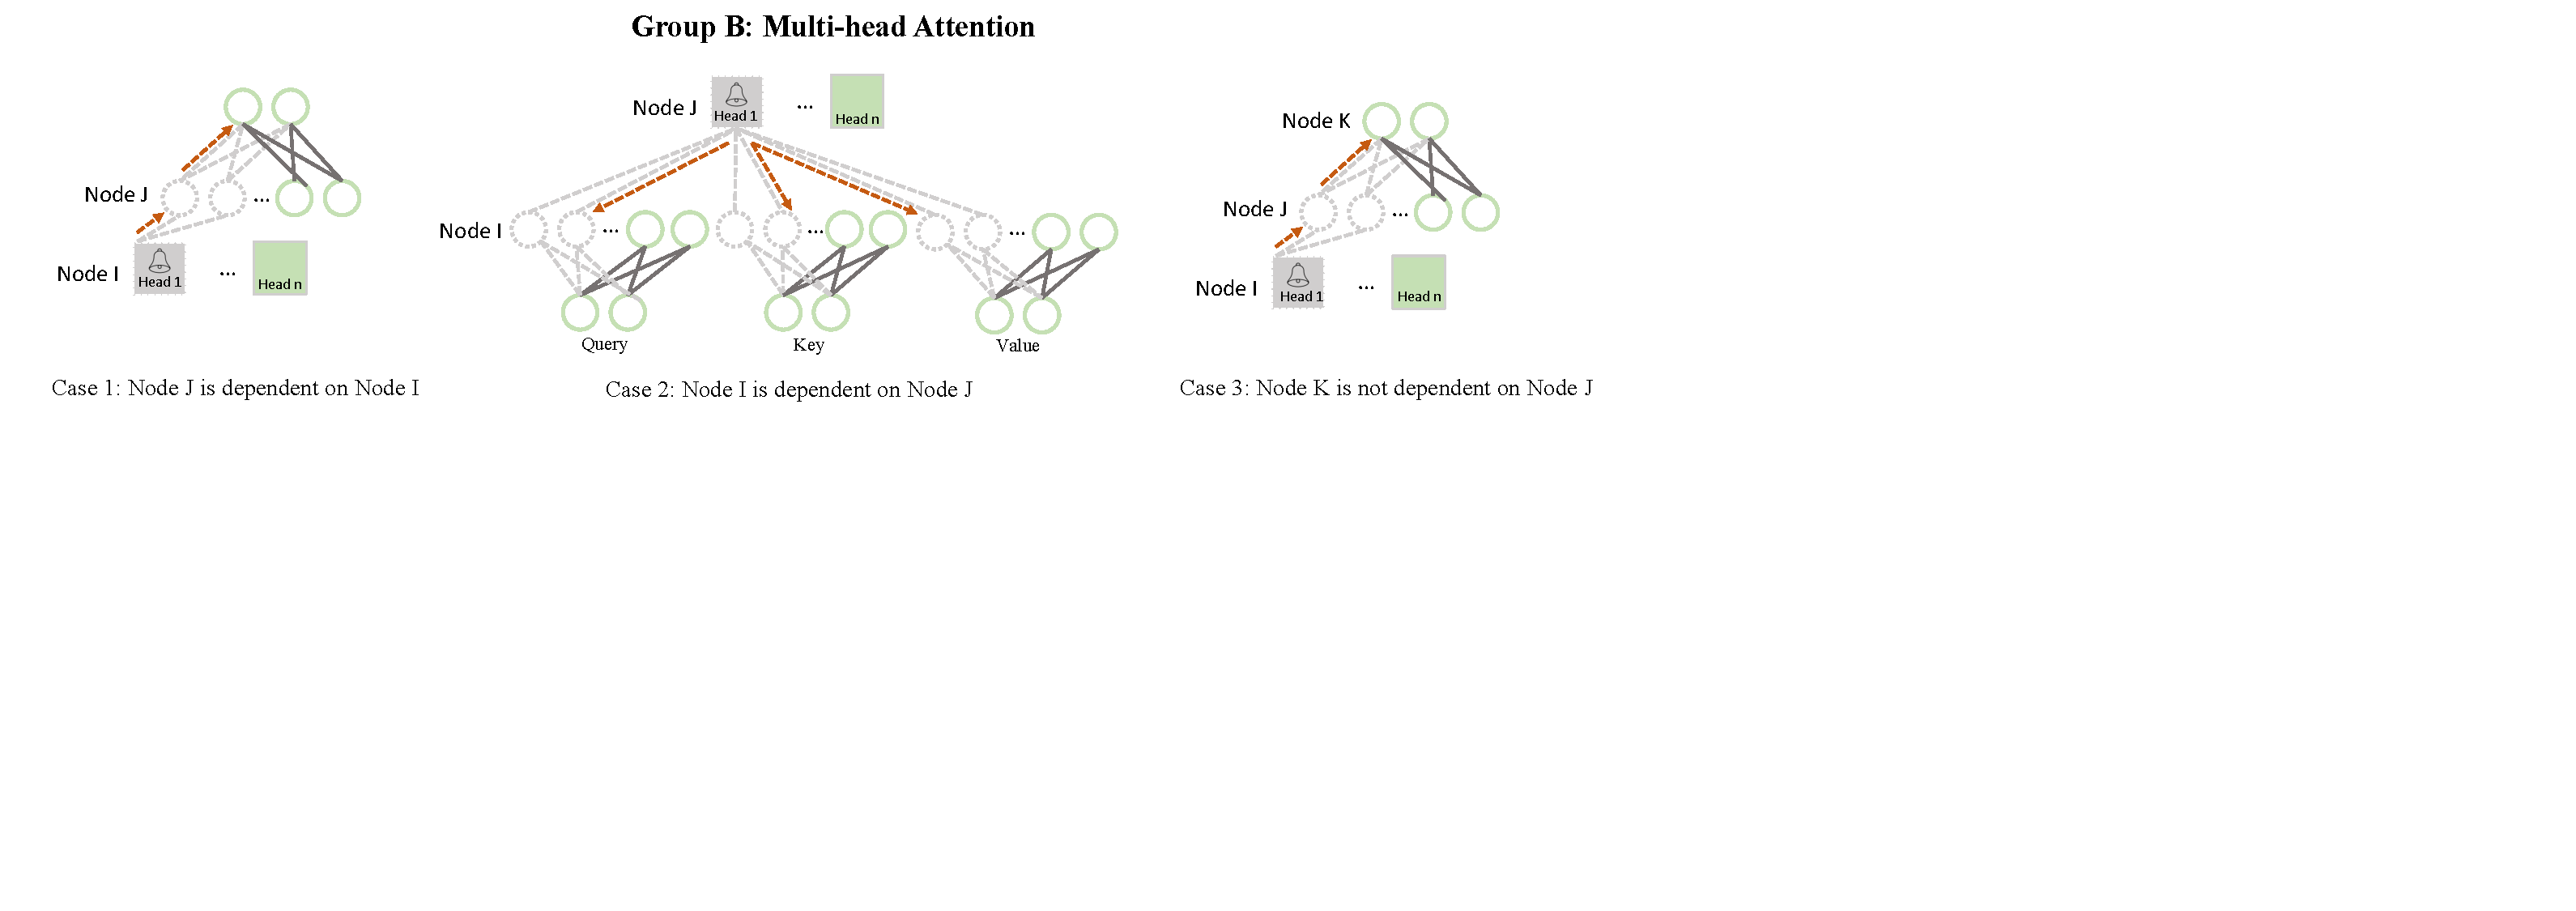
\includegraphics[width=\linewidth]{figures/rule_explanation.pdf}
    \caption{
        Illustrations of the two dependency rules. All the cases are extracted from the multi-head attention module.
    }
    \label{fig:rule}
\end{figure}
We provide a detailed explanation of the two dependency rules. It is important to note that these dependency rules do not pertain solely to the forward computation. Instead, they represent directional relationships that exist in both directions. For instance, removing a node in a subsequent layer may also result in the pruning of a node in the preceding layer. Recall the two dependency rules as follows:
\begin{equation}
     N_j \in \operatorname{Out}(N_i) \wedge \operatorname{Deg}^-(N_j) = 1 \Rightarrow N_j \text{ is dependent on } N_i \label{eq:depen}
\end{equation}
\begin{equation}
     N_i \in \operatorname{In}(N_j) \wedge \operatorname{Deg}^+(N_i) = 1 \Rightarrow N_i \text{ is dependent on } N_j \label{eq:depen_inv}
\end{equation}
where $N_i$ and $N_j$ are two neurons. $\operatorname{In}(N_i)$ and $\operatorname{Out}(N_i)$ represents all the neurons that point towards or point from $N_i$. $\operatorname{Deg}^-(N_i)$ and $\operatorname{Deg}^+(N_i)$ represents the in-degree and out-degree of neuron $N_i$. 

Figure \ref{fig:rule} serves as an illustration of the two dependency rules:
\begin{itemize}[leftmargin=*]
    \item In case 1, Node I and Node J satisfy the rule stated in Eq.\ref{eq:depen}. Consequently, Node J depends on Node I. When Node I is pruned, it is necessary to prune Node J as well.
    \item In case 2, Node I and Node J satisfy the rule Eq.\ref{eq:depen_inv}. Thus, Node I is dependent on Node J. If Node J is pruned, it becomes imperative to prune Node I as well.
    \item In case 3, Node J and Node K do not meet the requirement of Eq.\ref{eq:depen} due to the mismatch in $\operatorname{Deg}^-(N_k) \neq 1$. Thus, with Node J pruned, Node K would not be affected.
\end{itemize}

\section{Implementation Details} \label{sec:apx_implementation_details}
\subsection{For Pruning}
\paragraph{For the baseline}
Given the lack of previous work on the structural pruning of Large Language Models in a task-agnostic and low-resource setting, there is currently no existing baseline for our model. To provide a comprehensive demonstration of the effectiveness of LLM-Pruner, we employ two additional methods for evaluation, alongside the data-free pruning method. All of these methods are built upon the dependent groups identified in Section \ref{sec:dependency}:
\begin{itemize}[leftmargin=*]
    \item L2: We assess the importance of each group based on the magnitude of its weight matrix. 
    \item Random: This method involves randomly selecting certain groups for pruning.
\end{itemize}

\paragraph{For the `Block' Group.}

Based on the findings presented in Table \ref{fig:layer_sensitivity}, it is preferable to leave the first three layers and the final layer unchanged, as modifying parameters in those layers significantly impacts the model. Within each module, such as the MLP or the Multi-head Attention, the discovered groups are pruned based on a pre-set ratio. For instance, in the MLP layer of LLaMA-7B, we identified 11,008 groups, and with a 25\% pruning ratio, the module would prune 2,752 groups. It is worth noting that the pruning rate for the selected groups is higher than the pruning ratio for the parameters, as certain layers (e.g., the embedding layer and excluded layers mentioned) retain their parameters.
When aiming for a parameter pruning ratio of 20\%, we prune 25\% from Layer 5 to Layer 30. Similarly, for a 50\% parameter removal, we prune 60\% of the groups from Layer 4 to Layer 30. 


\paragraph{For the `Channel' Group.} The Group 'Channel' exhibits a resemblance to dimension pruning in the model, targeting the pruning of certain dimensions. In the case of the Query, Key, and Value projection in MHA, only the input dimension is pruned, while for the Output projection in MHA, only the output dimension is pruned. It is important to note that the entire dependency is established automatically, without any manual design involved. The `Channel' group operates in a complementary manner to the `Block Group'. In the `Channel' Group, the pruning ratio of the group equals to the pruning ratio of the parameters, as all weight matrices, including the embedding matrix, undergo pruning. Therefore, a 20\% pruning ratio of parameters implies pruning 20\% of the groups, while a 50\% pruning ratio implies pruning 50\% of the groups.

\iffalse{
\paragraph{For ChatGLM-6B}
For ChatGLM, we only prune the groups within the MLP layer due to our observation that pruning the groups within the MHA layer adversely affects the model's performance (See Figure \ref{fig:chatglm-mlp-head}). We are still exploring the underlying reason for this. Since ChatGLM-6b contains approximately 17\% of its parameters in the embedding layer and final prediction head, and the removal of parameters within MHA has a significant impact on the model, thus the pruning ratio for ChatGLM-6B is not as high as the one utilized in LLaMA and Vicuna. 

\begin{figure*}[h]
\centering
    \begin{subfigure}[b]{0.32\linewidth}
        \includegraphics[width=\linewidth]{figures/chatglm_ARC-e.pdf}
        \caption{ARC-e} \label{fig:chatglm-arce}
    \end{subfigure}
    \begin{subfigure}[b]{0.32\linewidth}
        \includegraphics[width=\linewidth]{figures/chatglm_ARC-c.pdf}
        \caption{ARC-c} \label{fig:chatglm-arcc}
    \end{subfigure}
    \begin{subfigure}[b]{0.32\linewidth}
        \includegraphics[width=\linewidth]{figures/chatglm_PIQA.pdf}
        \caption{PIQA} \label{fig:chatglm-piqa}
    \end{subfigure}
    \caption{Pruning groups in MHA or MLP in ChatGLM-6B}
    \label{fig:chatglm-mlp-head}
    \vspace{-5mm}
\end{figure*}
}\fi

\subsection{For Recovery Stage}
\begin{wraptable}{r}{4.0cm}
\vspace{-4mm}
\caption{Ablation: Tuning different modules in the recovery stage }\label{tbl:lora_tune_modules}
 \resizebox{\linewidth}{!}{%
    \begin{tabular}{l|cc}
        \toprule
        Module & WikiText $\color{teal}\downarrow$ & PTB $\color{teal}\downarrow$ \\
        \midrule
        ALL & 17.36 & 29.99 \\
        - MLP & 17.64 & 30.63 \\
        - MHA & 17.62 & 30.23\\
        \bottomrule
    \end{tabular}  
}%
\vspace{-2mm}
\end{wraptable}
We follow \cite{hulora} in our recovery stage. We set the rank $d$ to 8 in our experiment. The learning rate is set to 1e-4 with 100 warming steps. The batch size of training is selected from \{64, 128\} and the AdamW optimizer is employed in our experiment. The best training epoch we found is 2 epochs, as training with more epochs even has a negative impact on the model performance. We run our experiment on a single GPU with 24GB memory, using approximately 2.5 hours if RTX4090 is utilized. All the linear module is taken into account for efficient tuning. An ablation experiment for this is shown in Table \ref{tbl:lora_tune_modules}.


\section{More Analysis} 

\subsection{More Data for Recovery} 
Despite our primary experiments being conducted using  50k samples, we remain convinced that the inclusion of additional data could substantially enhance the recovery process, albeit at a considerably higher computational cost. Consequently, we conduct an experiment aimed at model recovery with more data, employing a dataset comprising 2.59 million samples~\cite{wu2023lamini}. The results are detailed in Table \ref{tbl:more_data}. From the results, it is evident that the performance of the compressed model closely approximates that of the base model, exhibiting only a marginal performance decrease of 0.89\%.

\begin{table}[h]
        \centering
        \caption{Model Recovery: 50k samples vs. 2.59M samples} \label{tbl:more_data}
        \resizebox{\linewidth}{!}{
        \begin{tabular}{l|c|ccccccc|c}
            \toprule
            \toprule
            Model & \#Samples &BoolQ & PIQA & HellaSwag & WinoGrande & ARC-e & ARC-c & OBQA & Average \\
            \midrule
            LLaMA-7B & - & 73.18 & 78.35 & 72.99 & 67.01 & 67.45 & 41.38 & 42.40 & 63.25 \\
            LLaMA-5.4B & 50k~\cite{alpaca} & 64.62 & 77.20 & 68.80 & 63.14 & 64.31 & 36.77 & 39.80 & 59.23 \\
            LLaMA-5.4B & 2.59M~\cite{wu2023lamini} & 76.57 & 77.37 & 66.60 & 65.82 & 70.62 & 40.70 & 38.80 & 62.36 \\
            \bottomrule
            \bottomrule
        \end{tabular}
        }
    \end{table}

\subsection{Pruning vs. Quantization}

Here, we conduct a comparative analysis of different compression techniques and illustrate that these techniques can be effectively combined with little performance degradation. We have chosen LLM.int8()~\cite{dettmers2022llm} as a representative example of quantization methods. Our results show that LLM.int8()  outperforms LLM-Pruner while LLM-Pruner enhances latency, reduces parameter size. 
When these two techniques are applied in tandem, they collectively reduce memory consumption and expedite inference, offering a balanced approach that combines the benefits of both methods.


\begin{table}[h]
        \centering
        \caption{Pruning and Quantization on LLaMA-7B}
        \resizebox{\linewidth}{!}{
        \begin{tabular}{l|ccc|ccccccc|c}
            \toprule
            \toprule
            Pruning Ratio & \#Param & Memory & Latency & BoolQ & PIQA & HellaSwag & WinoGrande & ARC-e & ARC-c & OBQA & Average \\
            \midrule
            LLaMA-7B & 6.74B & 12884.5MiB & 69.32s & 73.18 & 78.35 & 72.99 & 67.01 & 67.45 & 41.38 & 42.40 & 63.25 \\
            LLM.int8() & 6.74B & 6777.7MiB & 76.20s & 73.36 & 78.18 & 73.01 & 66.93 & 67.47 & 40.87 & 41.80 & 63.09 \\
            LLaMA-5.4B & 5.47B & 10488.4MiB & 58.55s &  76.57 & 77.37 & 66.60 & 65.82 & 70.62 & 40.70 & 38.80 & 62.36 \\
            LLaMA-5.4B + LLM.int8() & 5.47B & 5444.37MiB & 63.10s & 76.39 & 76.71 & 66.62 & 66.46 & 70.54 & 40.19 & 39.20 & 62.30 \\       
            \bottomrule
            \bottomrule
        \end{tabular}
        }
    \end{table}

\subsection{Global Pruning vs. Local Pruning}
we present a comparative analysis between global pruning and local pruning, where the pruning ratio is 20\% and the base model is LLaMA-7B. Global pruning refers to ranking all groups in the model together, whereas local pruning involves only ranking groups within the same module for pruning. The outcome of global pruning leads to varying widths across different layers and modules, whereas local pruning ensures uniformity across all layers.

Based on our experimental findings, we observed a slight advantage of local pruning over global pruning. We think this is because of the varying magnitudes in different layers or modules, which makes the importance scores incomparable between groups across different layers.

\begin{table}[h]
    \centering
    \vspace{-4mm}
    \caption{Results of global pruning and local pruning} \label{tbl:group_local_result}
    \resizebox{\linewidth}{!}{
    \begin{tabular}{l|cc|ccccccc|c}
        \toprule
        Method & WikiText2 $\color{teal}\downarrow$ & PTB$\color{teal}\downarrow$ & BoolQ & PIQA & HellaSwag & WinoGrande & ARC-e & ARC-c & OBQA & Average \\
        \midrule
        %$\text{Parameter}^2$ & 20.89 & 36.66 & 62.05 & 73.88 & 57.80 & 54.85 & 52.86 & 32.08 & 36.80 & 52.90 \\
        %Global & 21.05 & 32.79 & 69.63 & 72.42 & 63.59 & 65.51 & 55.68 & 34.81 & 37.80 & 57.06\\
        %\midrule
        $\text{Element}^1$ - local  & 19.09 & 34.21 & 57.06 & 75.68 & 66.80 & 59.83 & 60.94 & 36.52 & 40.00 & 56.69 \\% 57.06 & 75.68/75.08 & 50.69/66.80 & 59.83 & 60.94/50.04 & 31.91/36.52 & 29.20/40.00 & 56.69\\%63.52 & 72.69/72.58 &46.83/63.06 & 64.09 & 55.60/47.39 & 30.72/33.11 & 24.40/37.20 & 55.61 \\
        $\text{Element}^1$ - global & 20.84 & 32.86 & 63.15 & 73.23 & 63.31 & 66.38 & 55.85 & 35.49 & 38.00 & 56.49 \\
        \bottomrule
    \end{tabular}
    }
\end{table}

\subsection{Overfitting Phenomena in Post-Training} \label{sec:apx_overfit}
We present a comprehensive analysis of the overfitting issue in the recovery stage, as previously mentioned in Figure \ref{fig:tune_overfit}. Here the results cover all 9 datasets across various training steps. Based on the findings presented in Table \ref{tbl:overfit_all_datasets}, a noticeable trend emerges: the accuracy or generation quality initially shows improvement but subsequently experiences a slight decline. This pattern suggests that the recovery process is completed within a short period. And given that the training corpus is domain-constrained, more training epochs can result in overfitting to the specific dataset while potentially compromising the original capabilities of the language model.

\begin{table}[h]
    \centering
    \vspace{-5mm}
    \caption{The PPL and Accuracy on different training steps} \label{tbl:overfit_all_datasets}
    \resizebox{\linewidth}{!}{
    \begin{tabular}{l|cc|ccccccc|c}
        \toprule
        Step & WikiText2 $\color{teal}\downarrow$ & PTB$\color{teal}\downarrow$ & BoolQ & PIQA & HellaSwag & WinoGrande & ARC-e & ARC-c & OBQA & Average \\
        \midrule
        0 & 19.09 & 34.21 & 57.06 & 75.68 & 66.80 & 59.83 & 60.94 & 36.52 & 40.00 & 56.69 \\
        200 & 18.10 & 30.66 & 64.62 & \underline{77.20} & \underline{68.80} & 63.14 & 64.31 & 36.77 & 39.80 & 59.24 \\
        400 & 17.69 & \underline{30.26} & 63.00 & 76.66 & 68.75 & 63.54 & 64.39 & 37.20 & 40.60 & 59.16 \\
        600 & 17.69 & 30.57 & 66.24 & 76.28 & 68.52 & 63.85 & \underline{64.48} & 37.37 & 41.00  & \underline{59.68} \\
        800 & \underline{17.64} & 30.57 & 65.05 & 76.22 & 68.38 & 63.77 & 63.64 & 37.29 & 40.80 & 59.31 \\
        1000 & 17.67 & 30.60 & \underline{66.39} & 76.17 & 68.24 & \underline{64.17} & 63.05 & 37.37 & \underline{41.60} & 59.57\\
        1200 & 17.74 & 30.75 & 65.75 & 76.28 & 68.28 & 63.77 & 63.30 & 37.63 & 41.20 & 59.46 \\
        1400 & 17.88 & 30.85 & 64.34 & 76.28 & 68.31 & 63.85 & 63.47 & \underline{37.80} & 41.20 & 59.32 \\       
        \bottomrule
    \end{tabular}
    }
\end{table}

\subsection{Pruning with Large Rates} \label{sec:large_ratios}
Additionally, we conducted tests on LLaMA-7B and Vicuna-7B with 50\% parameters pruned. We observe a significant decrease in performance compared to the base model. However, the recovery stage proved to be beneficial, resulting in an improvement of approximately 7.39\%. Pruning a Language Model with such a high pruning rate remains a challenging task.

\begin{table}[h]
    \centering
    \vspace{-5mm}
    \caption{The PPL and Accuracy on LLaMA-7B} \label{tbl:llama_0.5_result}
    \resizebox{\linewidth}{!}{
    \begin{tabular}{ll|cc|ccccccc|c}
        \toprule
        Pruned Model & Method & WikiText2 $\color{teal}\downarrow$ & PTB$\color{teal}\downarrow$ & BoolQ & PIQA & HellaSwag & WinoGrande & ARC-e & ARC-c & OBQA & Average \\
        \midrule
        \multirow{7}{*}{\parbox{1.8cm}{Ratio = 50\% w/o tune}} & l2 & 39266.42 & 48867.85 & 55.11 & 53.59 & 27.03 & 49.49 & 26.43 & 29.01 & 34.40 & 39.29 \\%55.11 & 53.59/51.90 & 26.02/27.03 & 49.49 & 26.43/27.27 & 23.55/29.01 & 15.20/34.40 & 39.29\\%54.98 & 52.39/52.50 & 26.18/26.80 & 50.59 & 26.26/27.48 & 23.81/29.10 & 16.80/34.20 & 39.19\\
        & random & 3887.90 & 4337.27 & 46.79 & 53.37 & 27.50 & 50.59 & 28.07 & 27.90 & 30.00 & 37.75 \\
        \cmidrule{2-12}
        %& & similarity & & & 53.64 & 51.85/48.86 & 25.75/25.87 & 50.36 & 25.72/27.10 & 23.21/27.47 & 13.80/30.40 & 37.90\\
        & \channelname & 13891.92 & 16114.91 & 40.37 & 52.18 & 25.72 & 48.86 & 25.72 & 28.24 & 30.40 & 35.93 \\%40.37 & 52.18/49.95 & 25.64/25.72 & 48.86 & 25.72/26.39 & 21.84/28.24 & 14.20/30.40 & 35.93 \\
        \cmidrule{2-12}
        & Vector & 141.06 & \underline{236.24} & \underline{62.17} & 55.11 & 27.25 & 49.88 & 29.00 & 25.77 & 34.00 & 40.45 \\
        %& $\text{Element}^2$ & 115.58 & 278.36 & 59.72 & 59.47 & 27.40 & 50.12 & 29.12 & 24.57 & 31.00 & 40.20 \\
        & $\text{Element}^2$ & \underline{106.07} & 266.65 & 52.57 & \underline{60.45} & \underline{35.86} & 49.01 & 32.83 & 25.51 & \underline{34.80} & 41.58 \\
        & $\text{Element}^1$ & 112.44 & 255.38 & 52.32 & 59.63 & 35.64 & \underline{53.20} & \underline{33.50} & \underline{27.22} & 33.40 & \underline{42.13} \\% 52.32 & 59.63/59.63 & 30.63/35.64 & 53.20 & 33.50/32.83 & 24.66/27.22 & 18.40/33.40 & 42.13\\%62.17 & 59.03/57.40 & 29.55/32.97 & 50.36 & 33.80/31.94 & 20.31/26.37 & 12.60/30.60 & 42.19 \\
        %& $\text{Element}^{1+2}$ & 130.97 & 302.15 & 48.56 & \underline{59.96} & 33.98 & 52.09 & \underline{34.30} & 26.88 & \underline{34.00} & 41.40 \\
        \cmidrule{1-12}
        \multirow{5}{*}{\parbox{1.8cm}{Ratio = 50\% w/ tune}}
        & \channelname & 1122.15 & 1092.26 & 40.76 & 54.84 & 26.94 & 49.41 & 27.86 & 25.43 & 32.20 & 36.77 \\ %40.76 & 54.84/52.77 & 26.47/26.94 & 49.41 & 27.86/27.86 & 22.18/25.43 & 14.40/32.20 & 36.77 \\
        \cmidrule{2-12}
        & Vector & 43.47 & 68.51 & \bf 62.11 & 64.96 & 40.52 & 51.54 & 46.38 & 28.33 & 32.40 & 46.61 \\
        %& $\text{Element}^2$ & 40.13 & 72.75 & 60.37 & 66.97 & 42.31 & 52.01 & 46.17 & 26.54 & 34.60 & 47.00 \\
        & $\text{Element}^2$ & 45.70 & 69.33 & 61.47 & 68.82 & \bf 47.56 & \bf 55.09 & \bf 46.46 & 28.24 & 35.20 & \bf 48.98 \\
        & $\text{Element}^1$ & \bf 38.12 & \bf 66.35 & 60.28 & \bf 69.31 & 47.06 & 53.43 & 45.96 & \bf 29.18 & \bf 35.60 & 48.69 \\%60.28 & 69.31/67.95 & 38.71/47.06 & 53.43 & 45.96/40.15 & 24.66/29.18 & 22.60/35.60 & 48.69\\
        % 52.02 & 68.82/68.39 & 38.37/46.01 & 51.85 & 45.20/39.48 & 25.09/27.73 & 23.00/36.40 & 46.86 \\ %59.42 & 62.95/62.13 & 34.81/40.20 & 49.96 & 44.19/34.81 & 23.81/26.88 & 19.20/33.40 & 45.29 \\         
        % & Random Initialized - 0.2 & & & \\
        %& $\text{Element}^{1+2}$ & 39.02 & 71.45 & 61.56 & 68.72 & 46.62 & 52.64 & \bf 47.94 & \bf 29.27 & 35.40 & \bf 48.88\\
        \bottomrule
    \end{tabular}
    }
\end{table}
        
\begin{table}[h]
    \centering
    \vspace{-5mm}
    \caption{The PPL and Accuracy on Vicuna-7B} \label{tbl:vicuna_0.5_result}
    \resizebox{\linewidth}{!}{
    \begin{tabular}{ll|cc|ccccccc|c}
        \toprule
        Pruned Model & Method & WikiText2 $\color{teal}\downarrow$ & PTB$\color{teal}\downarrow$ & BoolQ & PIQA & HellaSwag & WinoGrande & ARC-e & ARC-c & OBQA & Average \\
        \midrule
         Ratio = 0\% & Vicuna-7B & 16.11 & 61.37 & 76.57 & 77.75 & 70.64 & 67.40 & 65.11 & 41.21 & 40.80 & 62.78 \\ %76.57 & 77.75/77.09 & 56.23/70.64 & 67.40 & 65.11/53.49 & 39.76/41.21 & 28.00/40.80 & 62.78 \\
        \cmidrule{1-12}
        \multirow{6}{*}{\parbox{1.8cm}{Ratio = 50\% w/o tune}} & l2 & 54516.03 & 66274.63 & 45.99 & 53.48 & 26.55 & 47.83 & 27.53 & 28.58 & 30.40 & 37.19 \\ %45.99 & 53.48/50.22 & 26.08/26.55 & 47.83 & 27.53/27.65 & 23.63/28.58 & 15.60/30.40 & 37.19\\
        & random & 17020.73 & 13676.54 & 48.17 & 53.43 & 27.31 & 50.43 & 26.30 & 29.78 & 30.20 & 37.95 \\ %48.17 & 53.43/52.07 & 26.35/27.31 & 50.43 & 26.30/27.06 & 22.27/29.78 & 15.40/30.20 & 37.95\\
        \cmidrule{2-12}
        & \channelname & 8360.30 & 10651.30 & 38.69 & 53.10 & 26.42 & 50.20 & 25.97 & 29.52 & 29.60 & 36.22 \\ % 38.69 & 53.10/48.86 & 25.78/26.42 & 50.20 & 25.97/25.59 & 22.18/29.52 & 13.20/29.60 & 36.22\\
        \cmidrule{2-12}
        & Vector & 189.87 & \underline{409.75} & \underline{62.14} & 55.33 & 26.99 & \underline{51.93} & 27.86 & 26.02 & 32.60 & 40.41 \\
        & Element$^2$ & \underline{143.85} & 427.77 & 53.76 & \underline{59.79} & \underline{34.86} & 50.28 & \underline{33.29} & 27.30 & 34.60 & \underline{41.98} \\ % 61.44 & 55.71 & 26.59 & 50.59 & 27.02 & 25.00 & 32.00 & 39.76 \\
        & Element$^1$ & 162.38 & 469.74 & 52.45 & 58.65 & 34.27 & 49.72 & 32.41 & \underline{28.75} & \underline{35.80} & 41.72 \\ %52.45 & 58.65/57.67 & 30.47/34.27 & 49.72 & 32.41/31.57 & 23.63/28.75 & 20.00/35.80 & 41.72\\
        %& Parameter$^{1+2}$ & 183.27 & 515.99 & 52.05 & 59.36 & 33.20 & 51.07 & 30.93 & 27.22 & 36.00 & 41.40 \\
        \cmidrule{1-12}
        & Channel & 206.23 & 526.89 & 62.11 & 58.38 & 32.29 & 51.22 & 33.08 & 24.06 & 30.20 & 41.62 \\
        \cmidrule{2-12}
        \multirow{3}{*}{\parbox{1.8cm}{Ratio = 50\% w/ tune}} 
        & Vector & 46.11 & 147.52 & \bf 62.14 & 64.91 & 39.80 & 50.91 & 47.77 & 27.30 & 32.60 & 46.49 \\
        & Element$^2$ & 42.99 & \bf 139.91 & 58.87 & \bf 69.48 & 46.38 & \bf 54.78 & 46.89 & 29.01 & 34.80 & 48.60 \\ %44.17 & 147.08 & 59.30 & 66.92 & 40.48 & 51.70 & 44.53 & 28.92 & 34.40 & 46.61 \\
        & Element$^1$  & \bf 41.64 & 143.74 & 62.08 & \bf 69.48 & \bf 46.79 & 54.54 & \bf 48.15 & \bf 29.78 & \bf 36.20 & \bf 49.57 \\
        %& Parameter$^{1+2}$  & 43.03 & 150.20 & 60.06 & 69.37 & 45.40 & 53.99 & 45.16 & 29.95 & 35.20 & 48.45 \\
    \bottomrule
    \end{tabular}
    }
\end{table}

\iffalse{
\begin{table}[h]
    \centering
    \vspace{-5mm}
    \caption{The PPL and Accuracy on Vicuna-7B v1.1} \label{tbl:vicuna_0.2_v1.1_result}
    \resizebox{\linewidth}{!}{
    \begin{tabular}{ll|cc|ccccccc|c}
        \toprule
        Pruned Model & Method & WikiText2 $\color{teal}\downarrow$ & PTB$\color{teal}\downarrow$ & BoolQ & PIQA & HellaSwag & WinoGrande & ARC-e & ARC-c & OBQA & Average \\
        \midrule
         Ratio = 0\% & Vicuna-7B &  \\
        \cmidrule{1-12}
        \multirow{6}{*}{\parbox{1.8cm}{Ratio = 20\% w/o tune}} & l2 & \\
        & random & \\
        \cmidrule{2-12}
        & \channelname & \\
        \cmidrule{2-12}
        & Vector &  27.03 & 45.26 &   \\
        & Element$^2$ & 23.81 & 43.52 & \\ 
        & Element$^1$ & 24.90 & 42.77 & \\ 
        \cmidrule{1-12}
        & Channel &  \\
        \cmidrule{2-12}
        \multirow{3}{*}{\parbox{1.8cm}{Ratio = 20\% w/ tune}} 
        & Vector &  \\
        & Element$^2$ & \\ 
        & Element$^1$  &  \\
    \bottomrule
    \end{tabular}
    }
\end{table}
}\fi

\section{Generations From Compressed Model}
Table \ref{tbl:visualization_llama}, \ref{tbl:visualization_vicuna}, \ref{tbl:chatglm_generate_en} and \ref{tbl:chatglm_generate_ch} show more examples of the models pruned by LLM-Pruner. We present the generation results of both the pruned model with post-training and without post-training. The absence of post-training allows us to better understand the information retained in the model. We include the results of ChatGLM-6B in two languages as it is a bilingual model.

\begin{table}[h]
    \centering
    \vspace{-4mm}
    \caption{Generated Examples from the Compressed LLaMA-5.4B } \label{tbl:visualization_llama}
    \resizebox{\linewidth}{!}{
    \tiny
    \begin{tabular}{p{0.8cm}|p{9.8cm}}
        \toprule
        Model & Generated Sentences \\
        \midrule
        \multirow{18}{*}{\parbox{0.8cm}{LLaMA w/ Tune}} & \underline{Neural Sequential Model, especially transformers,}  have become very popular due to their impressive performance in different areas. The neural network model can recognize the human voice more efficiently than speech recognition, and speech can be better distinguished. However, its high energy consumption has been the biggest problem. Many efforts have been made, such as minimizing the number of layers and the length of the neural network, but it has had no effect. The work is to develop a low-dimensional sound model which is suitable for the high frequency band of the speech. After reducing the ... \\
        \cmidrule{2-2}
        & \underline{AI can create a logo in seconds} or design a book cover, and they need to do it much faster than us humans can. So what are the implications that this has for branding design? Giving Creative Control to Algorithms. The first wave of ‘creative’ branding has come from designers and agencies submitting their creations to algorithms. They are algorithms that have been programmed to create, and are being asked to replace designers in the creative process. For example, in 1998 Google used a random process to select words and colours for their logo. Now, in \\
        \cmidrule{2-2}
        & \underline{What’s great about the holiday season}, is it provides us with the excuse we need to reconnect with the ones we have grown apart from. There are many people who I only talk to a couple of times per year during the year and never interact with them anymore, and while I’m completely okay with that – I feel they too should use Christmas as a great opportunity to get back in touch with people in their lives that maybe they were too busy to talk to before. If you are on good terms with a family member or friend, and you haven’t been talking to them lately due to how \\
        \midrule
        \multirow{16}{*}{\parbox{0.8cm}{LLaMA w/o Tune}} & \underline{Neural Sequential Model, especially transformers,} we designed them as a neural network that transforms input words to corresponding output. In our model, the 73 neural nodes are arranged in the form of L-shaped and are used to construct the two-dimensional lattice and form a sentence. This sentence is then transferred to the decoder to learn the words. Through 5.4.1 million repetitions, we can form a language model through the neural network we designed. With the help of a word-level data correction method, we made a strong progress in the recognition of human language. \\
        \cmidrule{2-2}
         & \underline{AI can create a logo in seconds}. You'll see a design in an instant and you'll be ?? that you're getting one the best logo designs around. The process is quick and easy and if you need it now you'll pay just a fraction of the cost for a professional logo designer. Why would I need a logo? It helps a brand stand out from the competition. It's the visual cue that people respond to - the logo. It's what makes you stop and look at the brand when you're walking by a street. Why invest in a logo? \\
        \cmidrule{2-2}
         & \underline{What’s great about the holiday season} is being with the people that you love, and the holidays are the perfect occasion to celebrate with the people that you love most. Being together with family and friends is one of those special occasions that can have a remarkable effect on how we perceive our lives, which is why they become some of the most cherished memories of our lifetimes. But holiday planning is more complex than a simple gathering. In fact, many families need professional advice to find the right way to handle the emotions involved. And that’s why planning, preparation, \\
        \bottomrule
    \end{tabular}
    }
\end{table}


\begin{table}[t]
    \centering
    \vspace{-4mm}
    \caption{Generated Examples from the Compressed Vicuna-5.4B} \label{tbl:visualization_vicuna}
    \resizebox{\linewidth}{!}{
    \tiny
    \begin{tabular}{p{0.8cm}|p{9.8cm}}
        \toprule
        Model & Generated Sentences \\
        \midrule
        \multirow{14}{*}{\parbox{0.8cm}{Vicuna w/ Tune}} & \underline{Last night we all danced together in the rain}, all our cares and worries forgotten. And as the sun began to rise, I looked into your eyes and knew that everything was going to be okay. That's the way it is now, forever and forever. I love you, my baby, and I always will. \\
        \cmidrule{2-2}
         & \underline{It fills me with such pride and joy} to be working along side her, learning from her and sharing our experiences, joys, and challenges as partners. Our bond is growing stronger each day and I can't help but feel grateful for the beautiful life she has brought into my own. To my loving wife, I love you more and more each day. I can't wait to spend the rest of my life with you and raising our future children together proyecting the light of Christ into the world. And to all of you reading this, I encourage you to take this seriously and consider your relationship with the one \\
        \cmidrule{2-2}
         & \underline{Meet me at midnight} tonight at the Bell Tower in town. Bring a torch, and we’ll take the treasure off the church’s hands, no matter the cost.’ With a deep sense of trepidation, Alaric finds himself agreeing to the plan. He spends the day getting everything he can from the village, preparing for the inevitable attack he’ll have to launch. When the day arrives, he and his companions mount their steeds and set off towards the towering keep of the temple. As they draw closer, the wind whispers \\
        \midrule
        \multirow{12}{*}{\parbox{0.8cm}{Vicuna w/o Tune}} & \underline{Last night we all danced together in the rain}. The water felt good on my face. The song played over and over, but I didn’t care. I just kept on dancing with you. I don’t know what to say. I’m not good with words. But I know that I’ve never felt this way before. With anyone. Not even myself. And I don’t want to let that feeling go. I don’t know what you feel, or what you want from me. But I know that this is real. And I don’t want to let it go \\
        \cmidrule{2-2}
          & \underline{It fills me with such pride and joy}, it’s like seeing my baby for the first time, and I just want to hold it close and never let it go. The thought that it might have to be put down one day breaks my heart. I want to do everything in my power to protect it, to keep it safe and give it the best life possible. But it’s not mine. It’s never been mine to keep. And I know that one day, sooner or later, it will have to be given away. I can’t help but feel a sense of responsibility that I don’t ... \\
        \cmidrule{2-2}
         & \underline{Meet me at midnight}, I promise you'll be the only one there. It's hard for me to believe, but I'm scared. I don't want to be alone tonight, but I know I have to be brave. Hurry down the hill, I'm waiting for you, I'll take you to a place that I know is safe. We won't be seen, nobody'll know. It's almost time for you to go. I don't want you to be late tonight. \\

        \bottomrule
    \end{tabular}
    }
\end{table}


\begin{table}[t]
    \centering
    \vspace{-4mm}
    \caption{Generated Examples from the Compressed ChatGLM-5.6B (English)} \label{tbl:chatglm_generate_en}
    \resizebox{\linewidth}{!}{
    \tiny
    \begin{tabular}{p{0.8cm}|p{9.8cm}}
        \toprule
        Model & Generated Sentences \\
        \midrule
        \multirow{14}{*}{\parbox{0.8cm}{ChatGLM w/ Tune}} & \underline{How to buy a cat?} It's important to understand that while it's understandable that you might be looking todnle a cat for yourself, adoption is a great way to bring home a furry friend without having to shop. Here are some things to consider before adoption: 1. First, make sure you know you're interested in Jr. or Vioness. This determines whether you're looking for a young adult cat or an older cat. 2.  research your options: Look up reputable cat owners or organizations that foster cats in your area. This will give you information on cat owners \\
        \cmidrule{2-2}
         & \underline{What is McDonald's?} McDonald's is a popular American fast-food restaurant chain that offers a variety of food and beverage items. The company was founded in 1940 by Richard and Maurice Mc Eu Eu in San Francisco, and the chain was originally called "McNugguggets." Today, McDonald's is known for its popular fast-food items such as McDonald's Drive-Thru, McChickens, and McFlurryrry. The company also offers a wide range of other food and beverage items such as Happy Endings, Big Macs, and ... \\
        \cmidrule{2-2}
         & \underline{What is Mean Square Error?} The Mean Square Error (MSE) is a measure of the difference between a target value and the best possible estimate of its true value, based on the data. It is calculated by taking the average difference between the actual value and the estimated value over the※ number of times the target value is repeated. \\
        \midrule
        \multirow{14}{*}{\parbox{0.8cm}{ChatGLM w/o Tune}} & \underline{How to buy a cat?} It's important to understand that adopting a cat from a shelter or organization is a valuable and responsible adoption option, as well as one that may be safer and more comfortable for you and your family. Additionally, it's important to read carefully before adopting to ensure that you choose a Cat who is suitable for you and your family. \\
        \cmidrule{2-2}
         & \underline{What is McDonald‘s?} McDonald's is a popular fast-food restaurant chain from United States known for its restaurant concepts such as McNugguggets, McFlurryrry, and McRibibs. The chain started in 1955 as a small operation operation called "Speedy McDonald's" in San Antonio, Texas and it quickly expanded and became a widely recognized and popular phenomenon in the country. Today, McDonald's is global icon known around the world. \\
        \cmidrule{2-2}
         & \underline{What is Mean Square Error?} Mean Square Error (MSE) is a measure of the accuracy of a function or a measurement when it is repeated and the result is expected to be within a certain range. It is calculated by taking the difference between two sets of measurements and measuring the difference squared. In simple terms, it means the mean sum of the errors over a given period of time or the difference between the actual and expected values of ... \\
        
        
        \bottomrule
    \end{tabular}
    }
\end{table}



\begin{CJK*}{UTF8}{gbsn}
\begin{table}[t]
    \centering
    \vspace{-4mm}
    \caption{Generated Examples from the Compressed ChatGLM-5.6B (Chinese)} \label{tbl:chatglm_generate_ch}
    \resizebox{\linewidth}{!}{
    \tiny
    \begin{tabular}{p{0.8cm}|p{9.8cm}}
        \toprule
        Model & Generated Sentences \\
        \midrule
        \multirow{16}{*}{\parbox{0.8cm}{ChatGLM w/ Tune}} & \underline{请给我推荐两个北京著名的景点} 北京著名的景点有很多,以下是两个:1. 颐和园:颐和园是北京的一座皇家园林,也是世界文化遗产。它是一座是一座结合了中国传统建筑和现代艺术的杰作,被誉为“万园之园”。颐和园内有很多建筑和景点,包括长廊、排排坐、佛香阁、万寿山等,非常适合漫步和参观。2. 故宫:故宫是中国古代皇宫,也是世界文化遗产,是北京的必去之地。它是世界上是世界上现存最大的、最完整的、最完整的、最著名的古代宫殿宫殿建筑之一。故宫内有很多建筑和景点,包括紫禁城 \\
        \cmidrule{2-2}
        & \underline{简单来说,相对论指出} 相对论是由爱因斯坦提出的一个关于时间和空间如何解释和变化的的理论,被称为狭义相对论。相对论认为,时间和空间并不是绝对的,而是相对的,也就是说,它们的测量值取决于观察者的惯性参照系。根据相对论,当物体以高速运动或以或以某种方式加速时,时间和空间的测量值会发生变化。最著名的是,时间和空间的测量值会“膨胀”,即随着物体运动,它们看起来会变得越来越长或越来越短。 \\
        \cmidrule{2-2}
        & \underline{如何健康的生活} 要保持健康的生活方式,可以参考以下建议:1. 定期锻炼:适量运动可以帮助增强身体健康,减轻压力,改善心情。建议每周至少进行3-5次有氧运动,如慢跑、快走、游泳、瑜伽等。2. 饮食均衡:控制饮食摄入量,摄入摄入适量、健康的蛋白质、碳水化合物、脂肪以及维生素和矿物质。3. 睡眠充足:充足的睡眠有助于恢复身体和大脑功能,提高身体免疫力。建议每晚睡眠7-8小时。4. 勤洗手:避免传染病毒。\\
        \midrule
        \multirow{16}{*}{\parbox{0.8cm}{ChatGLM w/o Tune}} & \underline{请给我推荐两个北京著名的景点} 北京著名的景点太多,以下是两个必去的景点:1. 故宫博物院: 故宫是世界上是世界上是世界上保存最完整的、最著名的宫殿建筑之一,也是中国历史文化名城和世界文化遗产。游客可以参观紫禁城紫禁城,欣赏到欣赏到大量的历史文物和艺术品。2. 长城: 长城是中国古代著名的防御工程之一,也是中国历史文化名城和世界文化遗产。游客可以参观长城的各种不同高度和不同用途的客房现代物流设施,还可以在长城上徒步。 \\
        \cmidrule{2-2}
        & \underline{简单来说,相对论指出} 相对论是由爱因斯坦提出的一组理论和概念,包括两个部分:狭义相对论和广义相对论。狭义相对论是描述在高速运动或缩短物体长度时,时间和空间如何弯曲的理论。它指出,当我们测量一个物体的长度或加速运动时,我们的测量结果观测到的是相对一个观察者观察者静止静止的物体长度或速度的尺子。这个理论解释了为什么光速是恒定不变的不变的。广义无味相对论是描述引力如何加速和改变物体的质量的。它指出,引力是由质量m和引力场引起的,两个物体引力场的中心的引力是 \\
        \cmidrule{2-2}
        & \underline{如何健康的生活} 想要过健康的生活可以参考以下建议: 1. 保持规律的规律的充足的睡眠:尽可能每晚每晚睡7-8个小时,保持规律的规律的睡眠时间有助于维持身体健康和精神状态。 2. 多运动:每天进行适量的运动有助于减轻压力和增强身体免疫力,建议每天进行适量的有氧运动和力量训练。 3. 饮食均衡:保持均衡的饮食,包括摄入足够的各种营养素和禁止过量摄入垃圾食品和饮料。 4. 减少不良习惯:尽可能减少不良习惯,如吸烟、酗酒和过度使用电子设备等。\\
        \bottomrule
    \end{tabular}
    }
\end{table}
\end{CJK*}
